\section{Introdução}

\subsection{Objeto de Estudo}
Esta apresentação irá tratar de um dispositivo de armazenamento de memória.

    \begin{figure}[H]
        \centering
        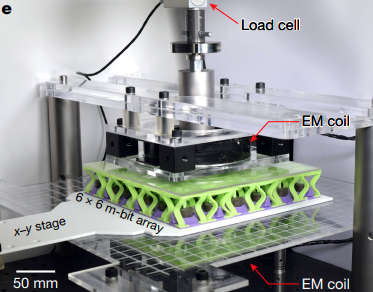
\includegraphics[scale = 0.5]{source/pictures/device.png}
        \caption{Imagem do dispositivo\cite{chen2021reprogrammable}.}
        \label{fig:device}
    \end{figure}

\subsubsection{O que é este dispositivo?}
    É um \textcolor{red}{dispositivo/sistema de memória} desenvolvido por Chen et al. capaz manipular informações de forma mecânica na estrutura do \textcolor{red}{material}\cite{coulais2021snappy}.\\ 

    Sendo capaz de:

    \begin{itemize}
        \item Codificar
        \item Armazenar
        \item Ler
        \item Alterar propriedades mecânicas do material
    \end{itemize}

    Para entendermos mais sobre este dispositivo, é necessário abordar os dois conceitos que envolvem este tema, que são: os metamateriais e os sistemas de armazenamento de dados. 

\subsection{Metamaterias}

\subsection{Sistemas de memória}
    Para melhor compreensão do funcionamento deste dispositivo, vamos construir uma analogia com outro dispositivo já conhecido que possui um funcionamento semelhante.

\subsubsection{Discos Rigidos}

    \begin{figure}[H]
        \centering
        \includegraphics[scale = 0.05]{source/pictures/hdd.png}
        \caption{Imagem de um disco rígido\cite{hdd-image}.}
        \label{fig:hdd}
    \end{figure}

    \begin{itemize}
        \item Apresenta funcionamento semelhante ao SDS\footnote{Snappy Data Storage}
        \item Utiliza \textit{bits} magneticos para manipular a informação
    
    \end{itemize}

    São sistemas de armazenamento de dados que apresentam funcionamento semelhante ao Snappy Data Storage, no entanto se baseia em um funcionamento eletromagnético para manipular as suas unidades básicas de memória, que são os bits.

\subsubsection{Funcionamento dos Discos Rígidos}

\begin{figure}[H]
    \centering
    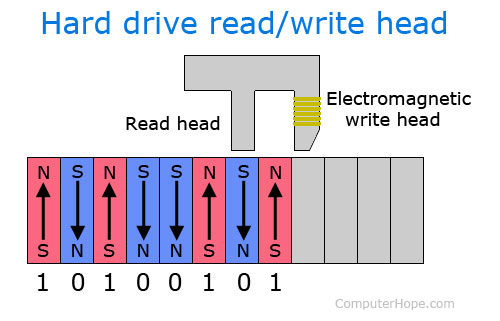
\includegraphics[scale = 0.5]{source/pictures/magnetic-media.jpg}
    \caption{Processo de gravação em um disco rígido\cite{hdd-image}.}
    \label{fig:hdd-recording}
\end{figure}

Para gravar informações em um disco rígido, o dispositivo através de um cabeçote eletromagnético magnetiza um bit e a sua polaridade determina o valor daquele bloco(\textit{building block})\cite{hdd-image}. Por exemplo, esta sequência de valores gravados significa o número 165 em código binário.\\ O bit é a unidade básica de memória deste sistemas, podendo assumir dois valores, sendo um ou zero. Este conceito será importante para entender o funcionamento do objeto de estudo deste trabalho.


